%!TEX root = ../TAMUTemplate.tex
%%%%%%%%%%%%%%%%%%%%%%%%%%%%%%%%%%%%%%%%%%%%%%%%%%%
%
%  New template code for TAMU Theses and Dissertations starting Fall 2016.
%
%  Author: Sean Zachary Roberson
%    Version 3.16.09
%  Last updated 9/12/2016
%
%%%%%%%%%%%%%%%%%%%%%%%%%%%%%%%%%%%%%%%%%%%%%%%%%%%

%%%%%%%%%%%%%%%%%%%%%%%%%%%%%%%%%%%%%%%%%%%%%%%%%%%%%%%%%%%%%%%%%%%%%%%
%%%                           SECTION II
%%%%%%%%%%%%%%%%%%%%%%%%%%%%%%%%%%%%%%%%%%%%%%%%%%%%%%%%%%%%%%%%%%%%%%

\chapter{\uppercase {Theoretical Framework}}
\label{ch:theoretical_framework}


\begin{comment}

Since the mid-1970s, the Standard Model (SM) of particle physics has been the leading theory describing three of the four known fundamental forces (not including gravity) as well as classifying all of the known elementary particles.
In 1961 Sheldon Glashow combined the electromagnetic and weak interactions in the first step towards creating the SM~\cite{GLASHOW1961579}.
Steven Weinberg and Abdus Salam~\cite{PhysRevLett.19.1264,salam} continued this work by adding in the Higgs mechanism~\cite{PhysRevLett.13.321,PhysRevLett.13.508,PhysRevLett.13.585} (more on this later) in 1967.
The model entered its current form in 1973-1974 with the introduction of the strong force and quantum chromodynamics.
The model can be broken down into the matter particles, spin $\frac{1}{2}$ fermions called leptons and quarks, the force mediators, spin 1 gauge bosons, and the spin-0 mediator of the Higgs field, all of which can be found in figure~\ref{fig:standard_model}.
Even during it's formative years, the SM's success at predicting new particles (i.e. the top quark in 1995) and describing the properties of known particles (i.e. $W^{\pm}$ to $Z^{0}$ mass ratio) is undeniable.


\begin{figure}[!hbt]
	%\scalebox{.45}{\input{StandardModel}}
	\centering
	\resizebox{0.55\textwidth}{!}{\input{StandardModel}}
	\caption{The Standard Model of particle physics. The model includes three generations of matter particles (leptons and quarks) as well as the gauge and Higgs bosons.}
	\label{fig:standard_model}
\end{figure}


\begin{figure}[bt]
	\centering
	\begin{subfigure}[t]{0.415\textwidth}
		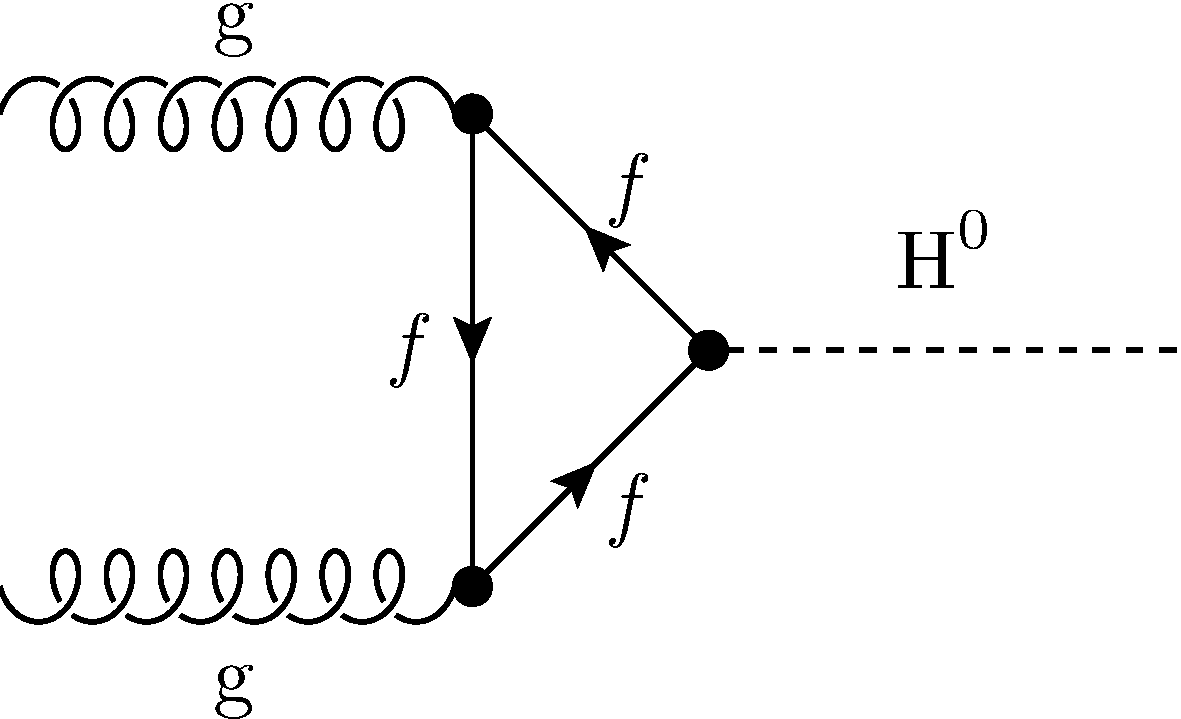
\includegraphics[width=\textwidth]{\figpath/FeynmanDiagrams/ggH.eps}
		\label{fig:ggH}
	\end{subfigure}%
	\begin{subfigure}[t]{0.415\textwidth}
		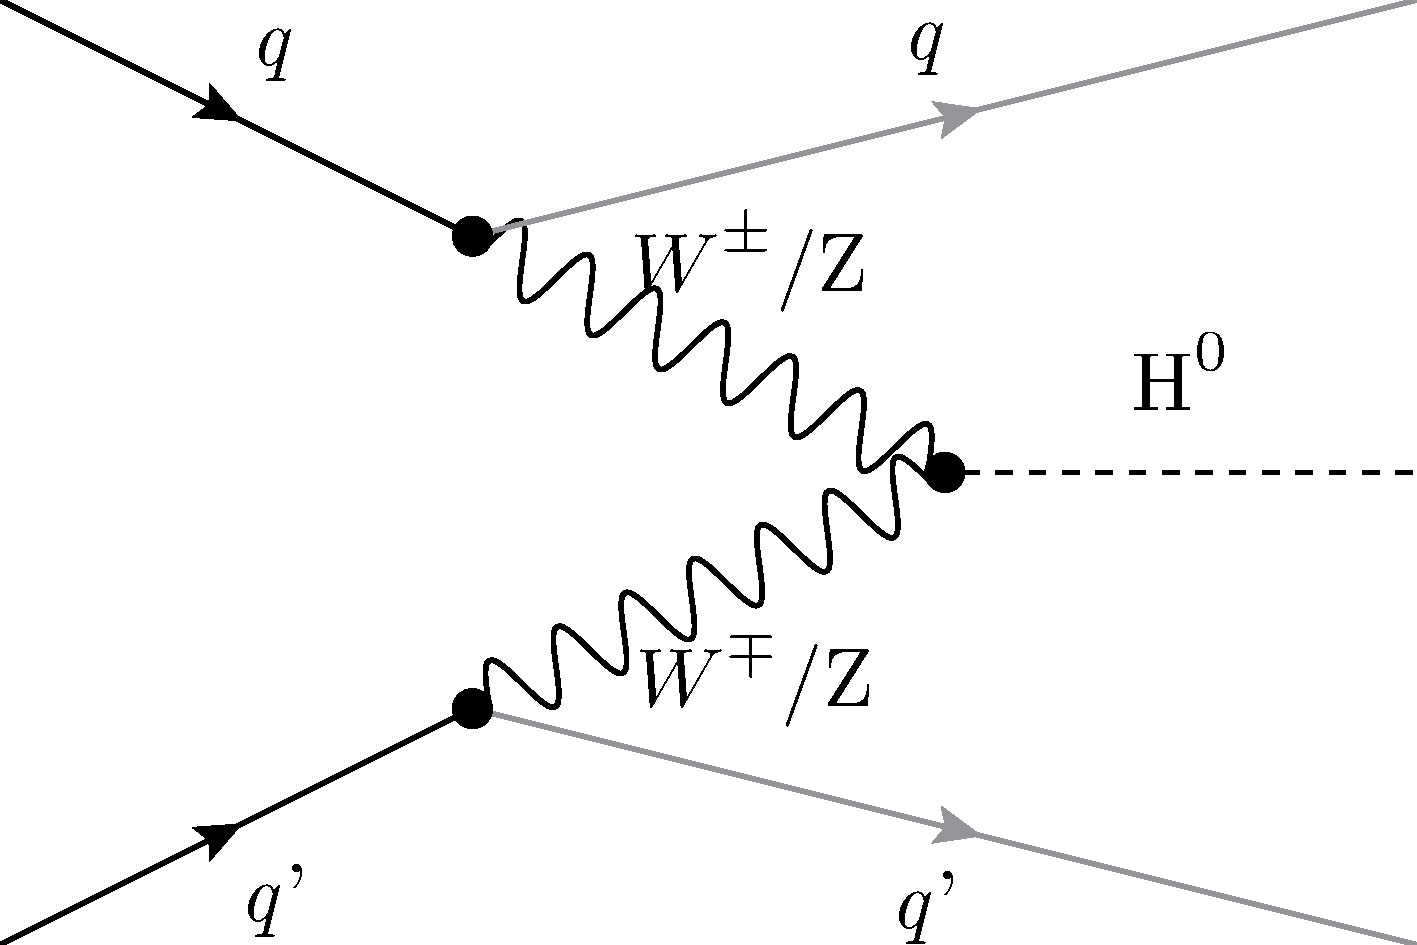
\includegraphics[width=\textwidth]{\figpath/FeynmanDiagrams/qqH.eps}
		\label{fig:qqH}
	\end{subfigure}

	\begin{subfigure}[t]{0.415\textwidth}
		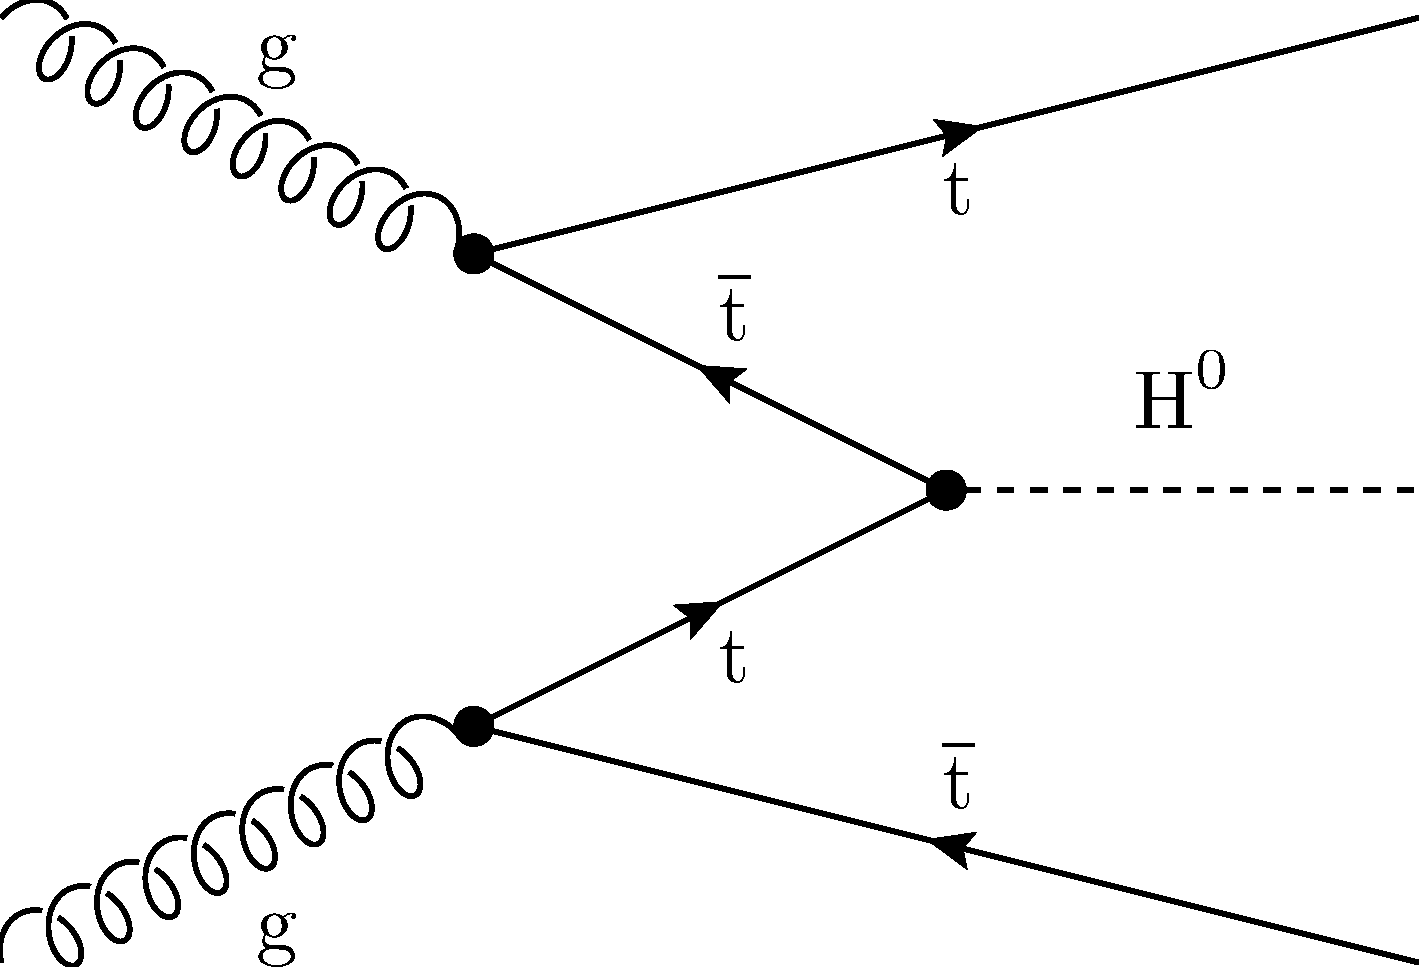
\includegraphics[width=\textwidth]{\figpath/FeynmanDiagrams/ttH.eps}
		\label{fig:ttH}
	\end{subfigure}%
	\begin{subfigure}[t]{0.415\textwidth}
		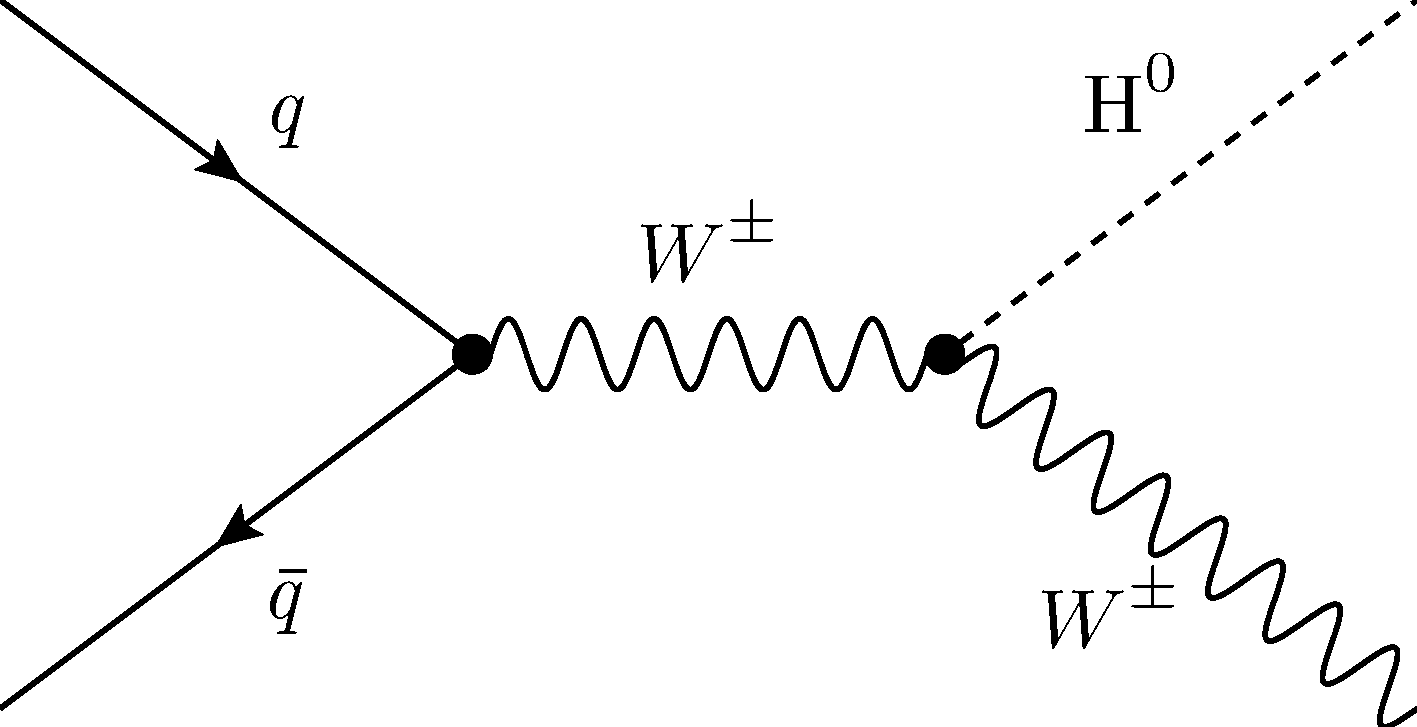
\includegraphics[width=\textwidth]{\figpath/FeynmanDiagrams/WH.eps}
		\label{fig:WH}
	\end{subfigure}
	\caption{Feynman diagrams for the four Higgs production mechanisms with associated $l{\nu}qq$ decays: gluon-gluon fusion (upper left), vector-boson fusion (upper right), \ttbar fusion (lower left), and associated production (lower right).}
	\label{fig:Higgs_WW_lnujj_feynman}
\end{figure}

\begin{figure}[!hbt]
	\centering
	\begin{subfigure}[t]{0.54\textwidth}
		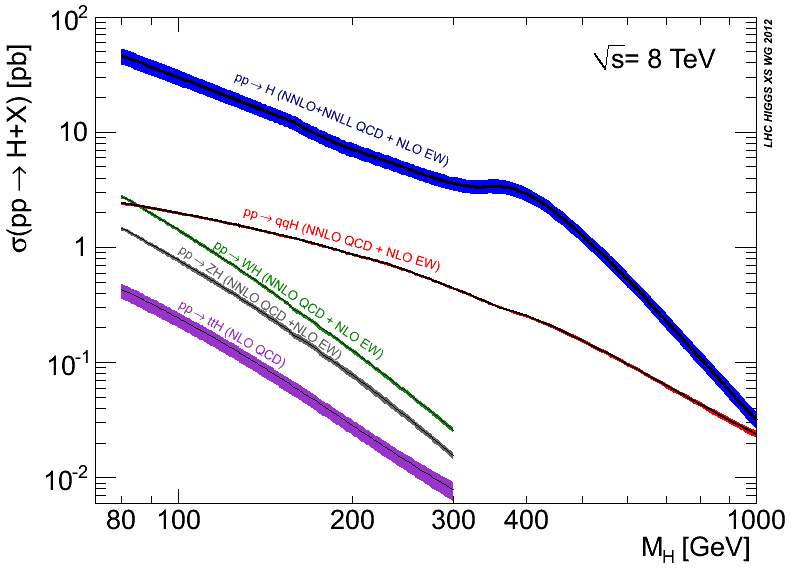
\includegraphics[width=\textwidth]{\figpath/Chapter1/Higgs_XS_8TeV.png}
		\label{fig:CERN_accelerator_complex}
	\end{subfigure}
	\begin{subfigure}[t]{0.41\textwidth}
		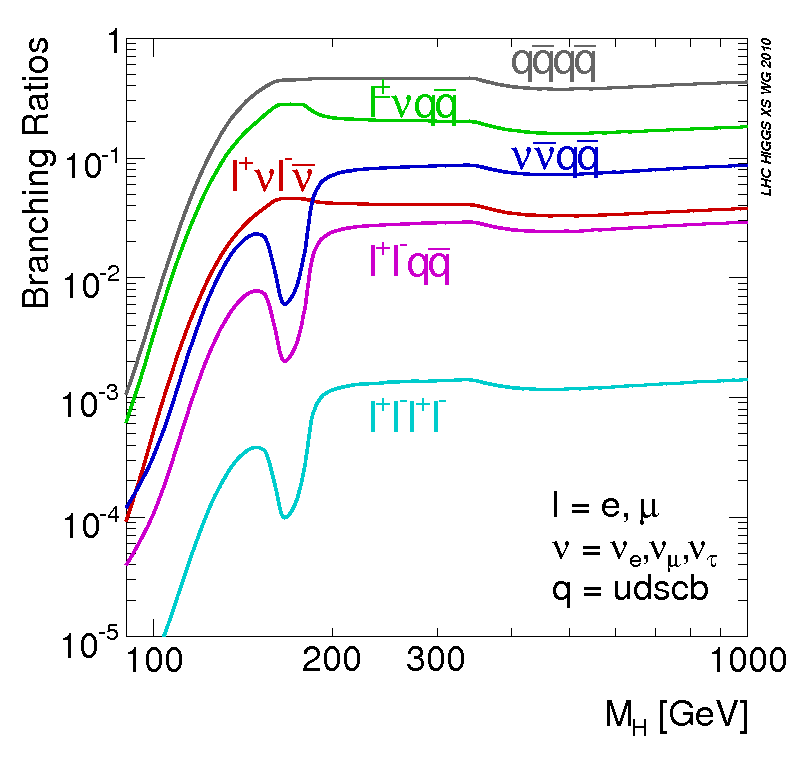
\includegraphics[width=\textwidth]{\figpath/Chapter1/Higgs_BR_4fermion.png}
		\label{fig:LHC_LEP_injection_complex}
	\end{subfigure}
	\caption{The Standard Model Higgs production cross sections at 8\tev (left) and WW branching ratios to four fermion final states (right).}
	\label{fig:Higgs_XS_and_BR}
\end{figure}

\end{comment}

\section{The Standard Model}
%\subsection{Leptons and Quarks}
%\subsection{Quantum Electrodynamics}
%\subsection{Electroweak Interaction}
%\subsection{Strong Interaction}
\subsection{Higgs Mechanism}

\section{Beyond the Standard Model}